\documentclass[11pt,a4paper]{article}
\usepackage[utf8]{inputenc}
\usepackage[T1]{fontenc}
\usepackage[margin=0.9in]{geometry}
\usepackage{graphicx}
\usepackage{xcolor}
\usepackage{booktabs}
\usepackage{hyperref}
\usepackage{titlesec}
\usepackage{fancyhdr}
\usepackage[most]{tcolorbox}
\usepackage{caption}
\usepackage{float}
\usepackage{mdframed}

% Define custom colors
\definecolor{primary}{RGB}{41, 128, 185}
\definecolor{secondary}{RGB}{142, 68, 173}
\definecolor{darkgray}{RGB}{52, 73, 94}
\definecolor{lightgray}{RGB}{236, 240, 241}

% Setup hyperref
\hypersetup{
    colorlinks=true,
    linkcolor=primary,
    urlcolor=primary,
    pdfborder={0 0 0}
}

% Custom section formatting
\titleformat{\section}
  {\Large\bfseries\color{primary}}
  {\thesection}{1em}{}[\vspace{-0.5ex}\color{primary}\titlerule]

\titleformat{\subsection}
  {\large\bfseries\color{darkgray}}
  {\thesubsection}{1em}{}

% Header and Footer
\pagestyle{fancy}
\fancyhf{}
\rhead{\textcolor{darkgray}{European Power Fair Value}}
\lhead{\textcolor{darkgray}{Quantitative Case Study}}
\rfoot{\thepage}
\renewcommand{\headrulewidth}{0.4pt}
\renewcommand{\footrulewidth}{0.4pt}

% Document Details
\title{\vspace{-1cm}\Huge\bfseries\color{primary} European Power Fair Value \\ \Large Forecasting Day-Ahead and Prompt Curve Translation}
\author{\large\textbf{Candidate:} Syed Ali Asad \hspace{1cm} \large\textbf{Email:} \href{mailto:saa110.work@gmail.com}{saa110.work@gmail.com}}
\date{\vspace{-0.5cm}}

\begin{document}

\maketitle
\thispagestyle{empty}

\begin{tcolorbox}[colback=lightgray, colframe=primary, title=\textbf{Executive Summary}]
This report outlines a practical, end-to-end prototype for forecasting hourly electricity prices in the German Day-Ahead market. We built a robust data pipeline that pulls live information directly from the official ENTSO-E API, automatically cleans it, and trains an ensemble of advanced machine learning models (Gradient Boosted Trees) to predict future prices. Finally, we translate these predictions into actionable trading signals, seamlessly integrating a language model (LLM) to mitigate risks from unexpected market events like power plant outages.
\end{tcolorbox}

\section{1. Data Pipeline \& Feature Engineering}
Data ingestion from the ENTSO-E API fetches Day-Ahead Prices, Actual Total Load, and Wind/Solar Forecasts. Quality Assurance (QA) rigorously handles DST transitions (23h/25h anomalous days), interpolates short gaps, and explicitly preserves true physical extreme/negative prices indicative of renewable oversupply (see Figure~\ref{fig:timeseries}).

To capture market dynamics, \textbf{14 core features} were engineered:
\begin{itemize}
    \setlength\itemsep{0em}
    \item \textbf{Temporal:} Hour of day, day of week, month, and weekend indicators.
    \item \textbf{Autoregressive Lags:} 24h \& 168h price lags, and 24h load lags.
    \item \textbf{Market Fundamentals:} Renewable penetration ratio (Wind+Solar / Load) and Net Load (Load $-$ Wind $-$ Solar).
    \item \textbf{Momentum / Volatility:} 24-hour rolling mean and standard deviation of prices.
\end{itemize}

\begin{figure}[H]
    \centering
    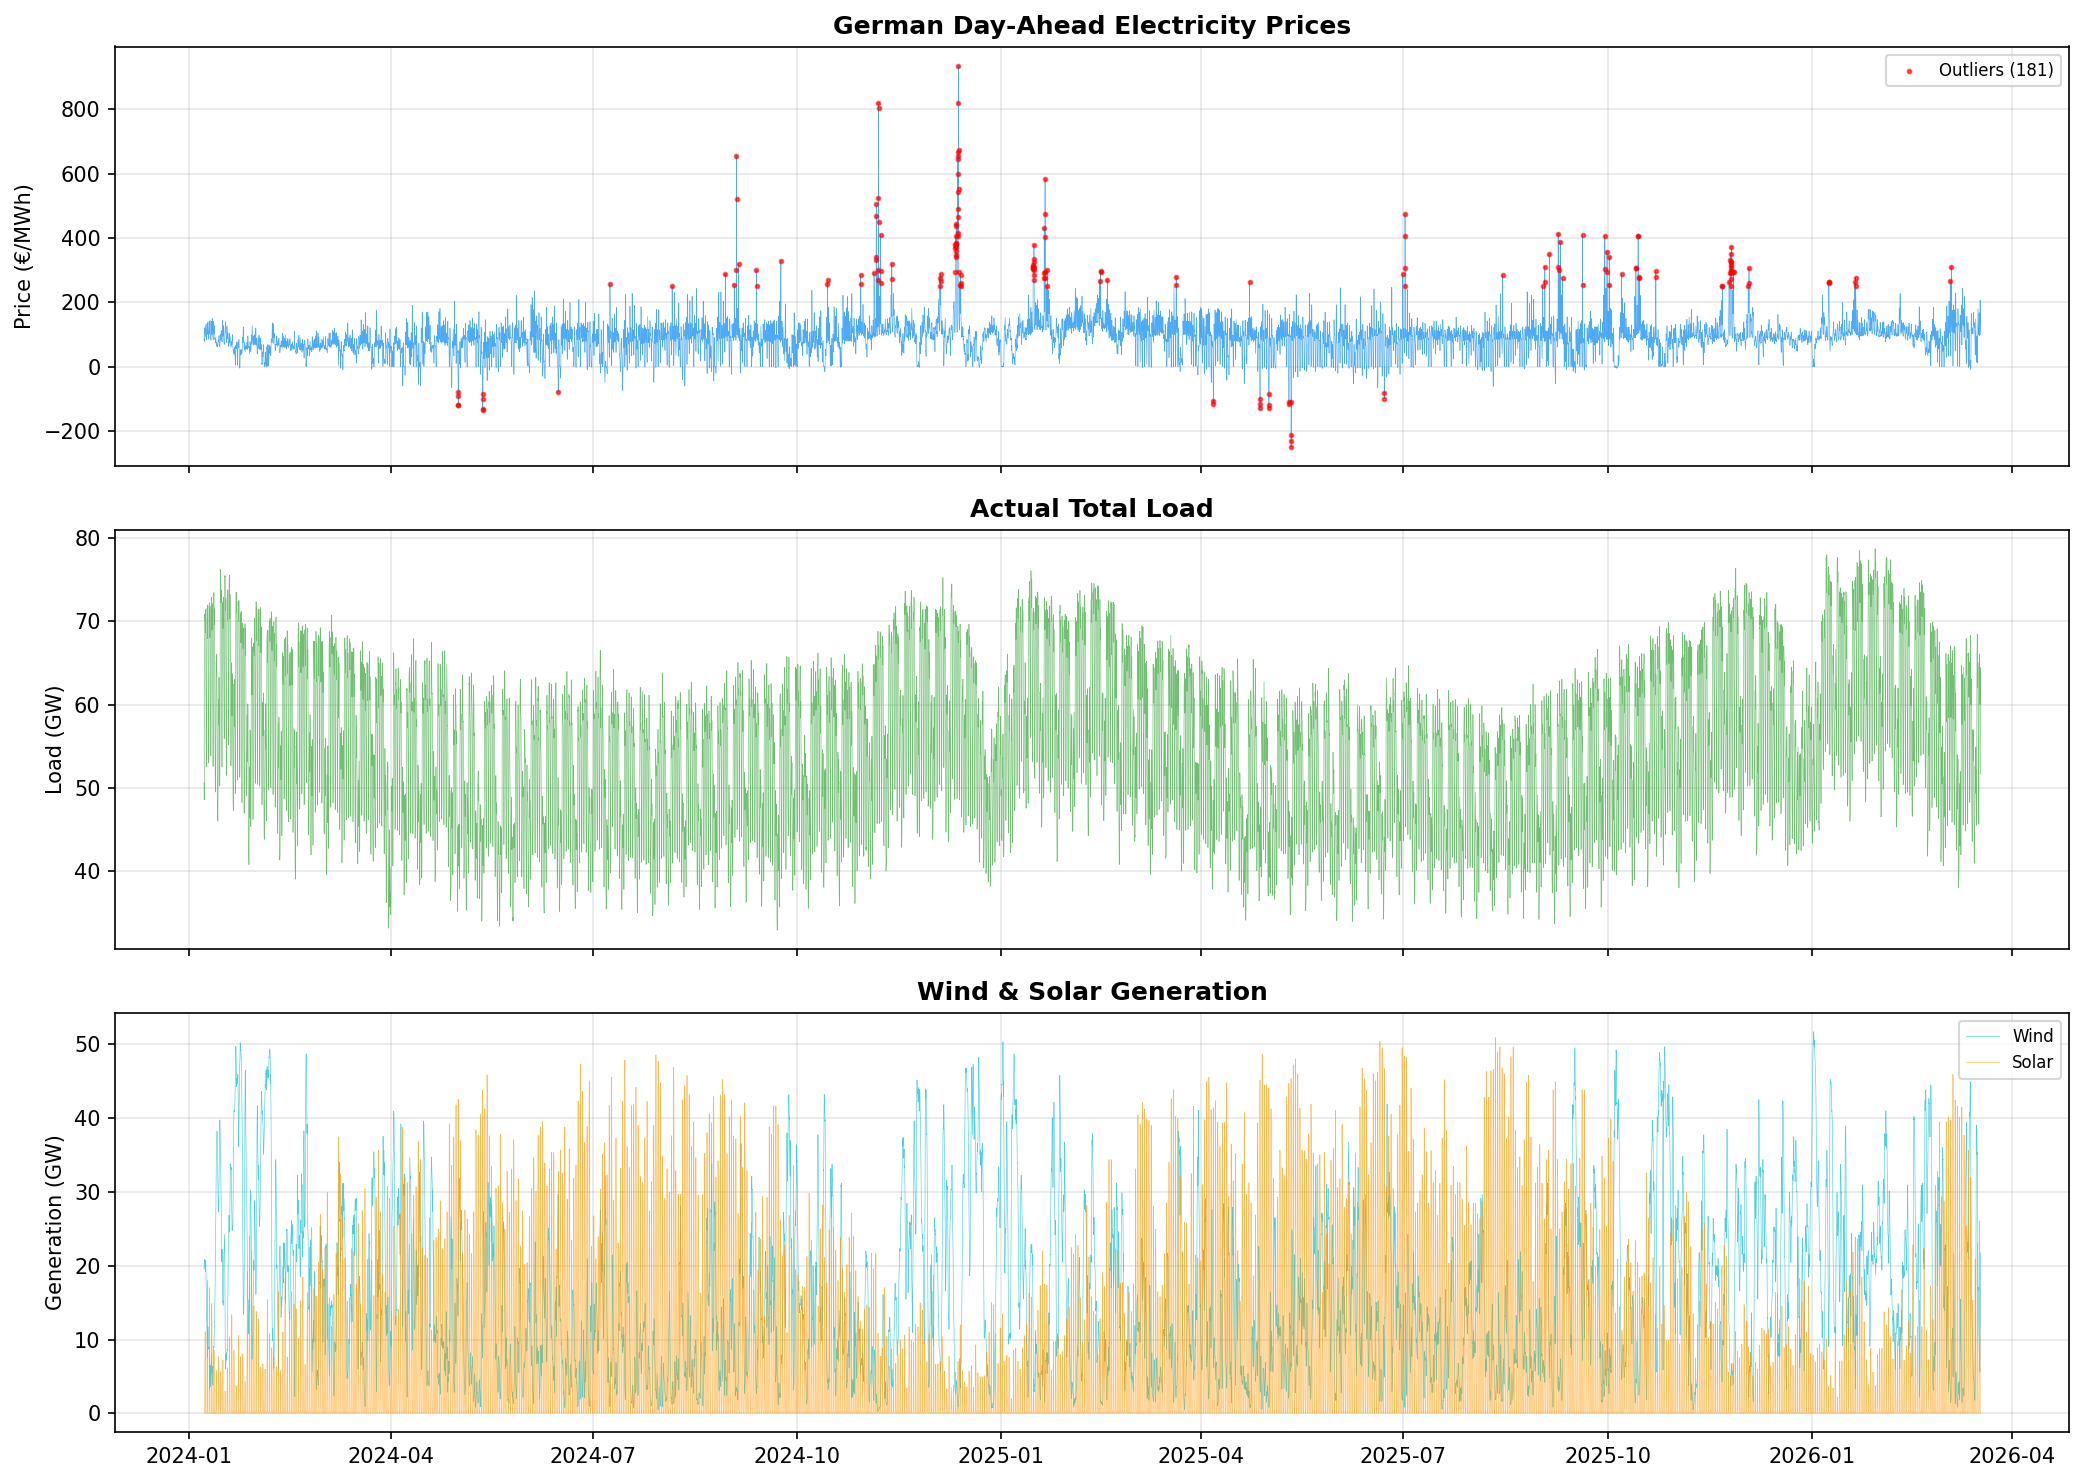
\includegraphics[width=0.85\textwidth]{../figures/price_timeseries.png}
    \vspace{-1em}
    \caption{Processed electricity price timeseries with QA-preserved extreme price events.}
    \label{fig:timeseries}
\end{figure}

\section{2. Forecasting \& Validation Rigor}
A suite of progressively advanced models was tested explicitly across an expanding 60-day rolling window to prevent lookahead bias. Symmetric Mean Absolute Percentage Error (sMAPE) natively handles instances of zero or negative prices (see Table~\ref{tab:metrics}).

\begin{itemize}
    \setlength\itemsep{0em}
    \item \textbf{Baseline Models:} Naive Persistence (Same-hour yesterday) and Ridge Regression (ARX).
    \item \textbf{Advanced Models:} LightGBM, XGBoost, and CatBoost configured to output robust probabilistic quantiles (q10, q50, q90).
    \item \textbf{Ensemble Strategy:} The Weighted Ensemble dynamically drops underperforming architectures, blending the Top 3 models (XGBoost, LightGBM, CatBoost) via inverse-RMSE weighting. It achieves optimal Directional Accuracy (83.3\%) and reduces out-of-sample variance.
\end{itemize}

\subsection{End-to-End Validation Metrics}
\vspace{-0.5em}
\begin{table}[H]
    \centering
    \small
    \begin{tabular}{lrrr}
        \toprule
        \textbf{Model} & \textbf{sMAPE (\%)} & \textbf{MAE (€/MWh)} & \textbf{Dir.Acc (\%)} \\
        \midrule
        Naive Persistence (Baseline) & 30.92\% & 24.23 & 79.8\% \\
        Ridge Regression (Baseline) & 24.85\% & 16.64 & 85.9\% \\
        Linear Regression (OLS) & 21.58\% & 15.48 & 83.5\% \\
        LightGBM & 16.84\% & 11.36 & 82.9\% \\
        XGBoost & 16.39\% & 10.88 & 82.1\% \\
        CatBoost & 16.93\% & 11.44 & 80.8\% \\
        \textbf{Ensemble (Final)} & \textbf{16.46\%} & \textbf{10.92} & \textbf{83.3\%} \\
        \bottomrule
    \end{tabular}
    \caption{End-to-End Validation Metrics for the 60-day out-of-sample period.}
    \label{tab:metrics}
\end{table}

\subsection{Feature Ablation Study}
Adding fundamentally-driven data (load or wind/solar) independently improves predictive error by $\sim$7\%. The full 14-feature engine explicitly yields the most optimal predictive power, as demonstrated in Figure~\ref{fig:ablation}.

\vspace{-0.5em}
\begin{figure}[H]
    \centering
    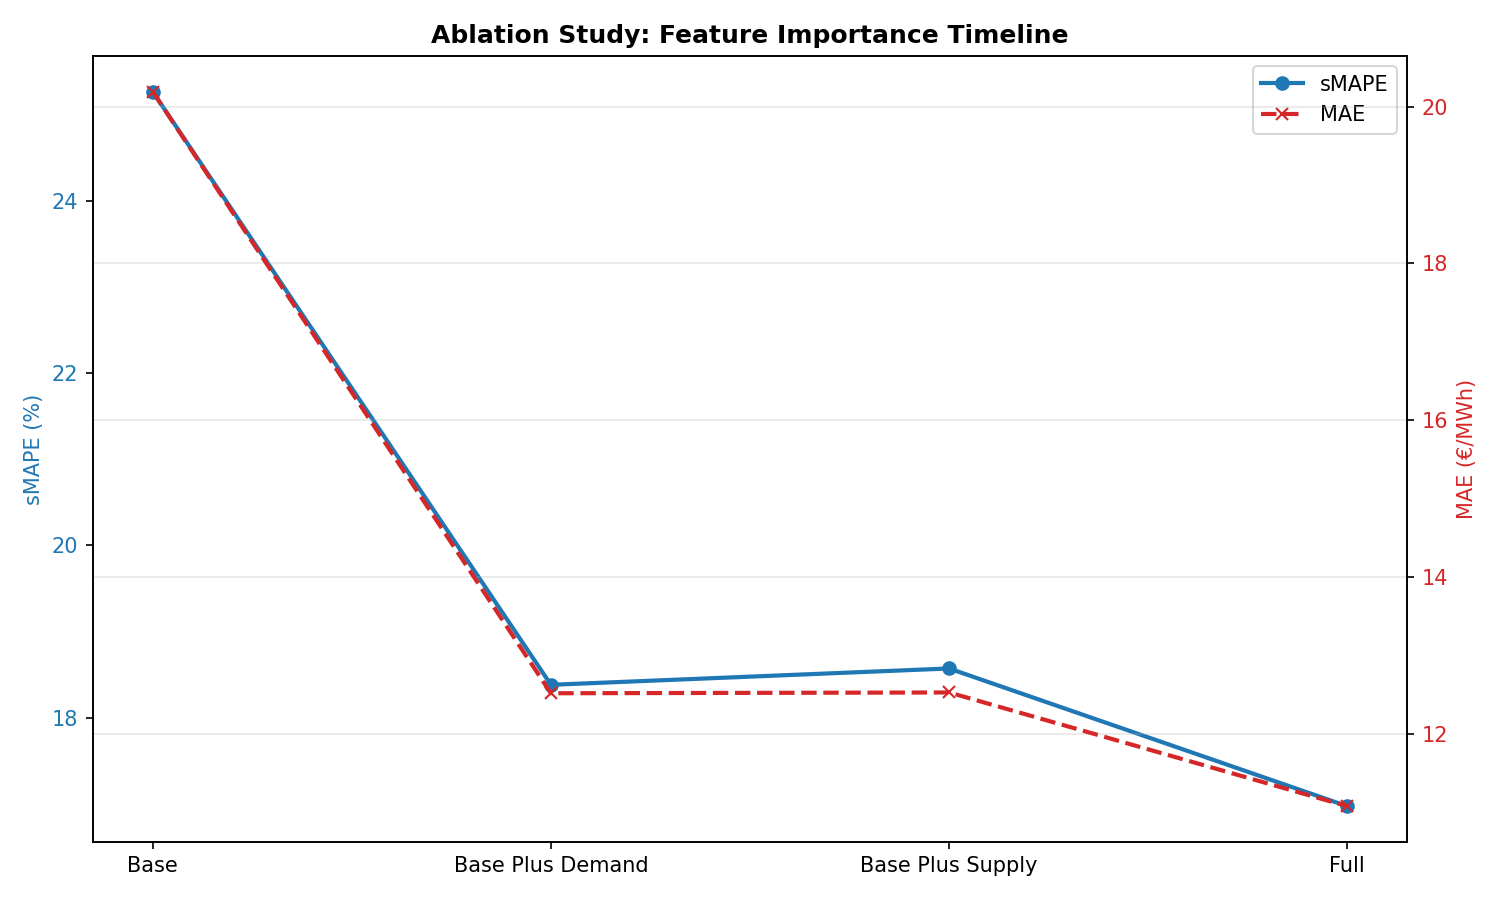
\includegraphics[width=0.7\textwidth]{../figures/ablation_chart.png}
    \vspace{-0.5em}
    \caption{Feature Impact on Model Accuracy}
    \label{fig:ablation}
\end{figure}

\section{3. Prompt Curve Translation}
Targeting DA-to-Curve positioning, the hourly ensemble forecasts are aggregated into forward Baseload and Peakload averages for the prompt week. The \texttt{curve\_translator.py} module extracts a \textbf{Risk Premium (RP)} against mocked forward prices.

\begin{itemize}
    \setlength\itemsep{0em}
    \item \textbf{Execution:} A \texttt{Strong Buy} / \texttt{Strong Sell} conviction is generated when the traded forward price falls entirely outside the ensemble model's 10th-90th percentile bounds (see Figure~\ref{fig:curve}).
    \item \textbf{Invalidation Criteria:} Signals are explicitly rejected if (1) confidence intervals are too wide, (2) actual prices hit extreme regimes ($>$\$200$ or $<-\$10$), or (3) the RP is too small (<€2/MWh).
\end{itemize}

\begin{figure}[H]
    \centering
    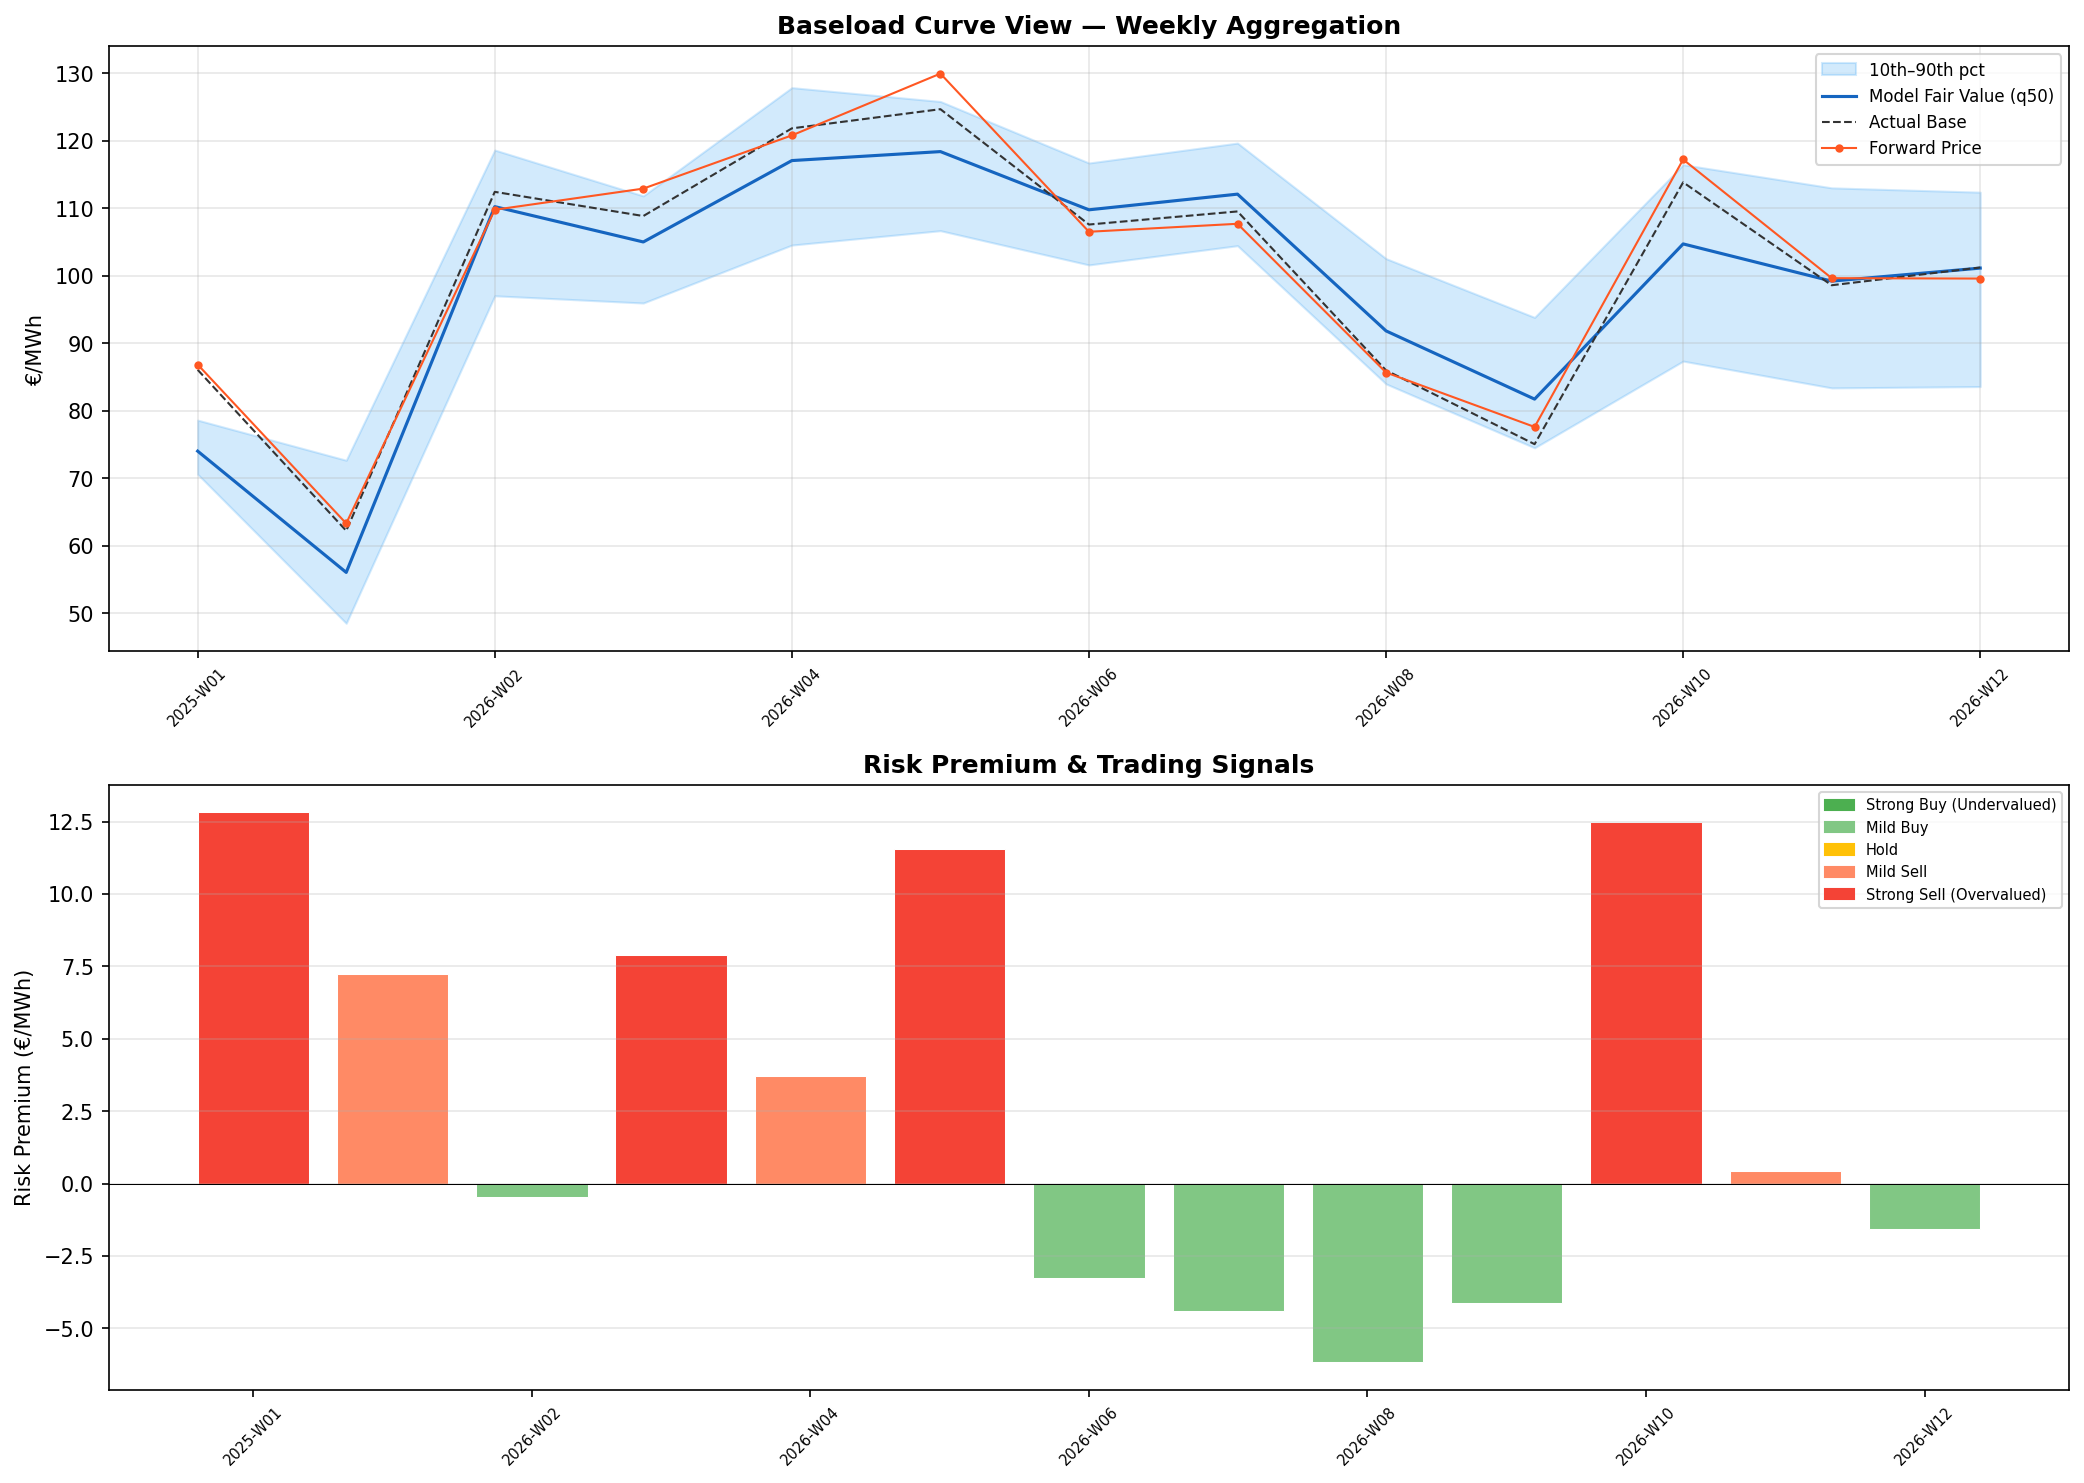
\includegraphics[width=0.85\textwidth]{../figures/curve_view.png}
    \vspace{-0.5em}
    \caption{Predicted Fair Value vs. Forward Prices demonstrating generated signal convictions.}
    \label{fig:curve}
\end{figure}

\section{4. Programmatic AI/LLM Integration}
To streamline quantitative workflows with unstructured fundamental events and mitigate operational risks:

\vspace{0.5em}
\begin{mdframed}[linecolor=primary, linewidth=1.5pt, backgroundcolor=lightgray!30]
\textbf{1. REMIT UMM Parsing (\texttt{remit\_parser.py})}\\
Electricity markets are heavily driven by largely unexpected supply outages. This module programmatically queries an LLM to read subjective, unformatted text about Planned Maintenance or Extreme Weather alerts and parses them into structured relevance scores. \textbf{Crucially, the LLM determines if an event is severe enough (e.g., "Generation Outage") to explicitly invalidate statistical trading signals.}
\end{mdframed}

\vspace{0.5em}

\begin{mdframed}[linecolor=secondary, linewidth=1.5pt, backgroundcolor=lightgray!30]
\textbf{2. QA Health Reporting (\texttt{qa\_health\_report.py})}\\
An automated daily system uses an LLM to read through execution logs and synthetically generate a human-readable morning briefing summary of data quality, model metrics, and active trading signals.
\end{mdframed}

\vspace{0.5em}
\noindent \textbf{Project Artifacts Map:}
\begin{itemize}
    \setlength\itemsep{0em}
    \item \texttt{docs/report/report.tex}: Strategic briefing (This document)
    \item \texttt{main.py} \& \texttt{README.md}: Unified orchestrator and environment setup
    \item \texttt{src/}: Codebase containing data ingest, QA, modeling, and translation logic
\end{itemize}

\end{document}
